\documentclass[french]{beamer}

\usepackage[utf8]{inputenc}
\usepackage[T1]{fontenc}
\usepackage{lmodern}
\usepackage{amsmath, amssymb,amsfonts}
\usepackage{mathrsfs}
\usepackage{calc}
\usepackage{graphicx}
\usepackage{babel}
\usepackage{tikz}
\usetikzlibrary{arrows,shapes,calc}
\tikzstyle{every picture}+=[remember picture]
\tikzstyle{na} = [baseline=-.5ex]
%\usepackage[sectionbib,square]{natbib}
\input{macros/macros}
\input{macros/macros-ph}
\newdimen\pgfex
\newdimen\pgfem
\usetikzlibrary{arrows,shapes,shadows,scopes}
\usetikzlibrary{positioning}
\usetikzlibrary{matrix}
\usetikzlibrary{decorations.text}
\usetikzlibrary{decorations.pathmorphing}

\usetikzlibrary{arrows,shapes}

\definecolor{lightgray}{rgb}{0.8,0.8,0.8}
\definecolor{lightgrey}{rgb}{0.8,0.8,0.8}

\definecolor{lightred}{rgb}{1,0.8,0.8}
\definecolor{lightgreen}{rgb}{0.7,1,0.7}
\definecolor{darkgreen}{rgb}{0,0.5,0}
\definecolor{darkblue}{rgb}{0,0,0.5}
\definecolor{darkyellow}{rgb}{0.5,0.5,0}
\definecolor{lightyellow}{rgb}{1,1,0.6}
\definecolor{darkcyan}{rgb}{0,0.6,0.6}
\definecolor{lightcyan}{rgb}{0.6,1,1}
\definecolor{darkorange}{rgb}{0.8,0.2,0}
\definecolor{notsodarkred}{rgb}{0.8,0,0}
\definecolor{darkred}{rgb}{0.5,0,0}

\definecolor{notsodarkgreen}{rgb}{0,0.7,0}

%\definecolor{coloract}{rgb}{0,1,0}
%\definecolor{colorinh}{rgb}{1,0,0}
\colorlet{coloract}{darkgreen}
\colorlet{colorinh}{red}
\colorlet{coloractgray}{lightgreen}
\colorlet{colorinhgray}{lightred}
\colorlet{colorinf}{darkgray}
\colorlet{coloractgray}{lightgreen}
\colorlet{colorinhgray}{lightred}

\colorlet{colorgray}{lightgray}
\colorlet{colorhl}{blue}


\tikzstyle{boxed ph}=[]
\tikzstyle{sort}=[fill=lightgray, rounded corners, draw=black]
\tikzstyle{process}=[circle,draw,minimum size=15pt,fill=white,font=\footnotesize,inner sep=1pt]
%\tikzstyle{black process}=[process, draw=blue, fill=red,text=black,font=\bfseries]
\tikzstyle{gray process}=[process, draw=black, fill=lightgray]
\tikzstyle{highlighted process}=[current process, fill=gray]
\tikzstyle{process box}=[fill=none,draw=black,rounded corners]
%\tikzstyle{current process}=[process, draw=black, fill=lightgray]
\tikzstyle{current process}=[process,fill=blue]
\tikzstyle{hl process}=[process,fill=blue!30]
\tikzstyle{tick label}=[font=\footnotesize]
\tikzstyle{tick}=[densely dotted] %-
\tikzstyle{hit}=[->,>=angle 45]
\tikzstyle{selfhit}=[min distance=50pt,curve to]
\tikzstyle{bounce}=[densely dotted,>=stealth',->]
\tikzstyle{ulhit}=[draw=lightgray,fill=lightgray]
\tikzstyle{pulhit}=[fill=lightgray]
\tikzstyle{bulhit}=[draw=lightgray]
\tikzstyle{hl}=[very thick,colorhl]
\tikzstyle{hlb}=[very thick]
\tikzstyle{hlhit}=[hl]
%\tikzstyle{hl2}=[hl]
%\tikzstyle{nohl}=[font=\normalfont,thin]

\tikzstyle{update}=[draw,->,dashed,shorten >=.7cm,shorten <=.7cm]

\tikzstyle{unprio}=[draw,thin]%[double]
%\tikzstyle{prioW}=[draw,thick,-stealth]%[double]
\tikzstyle{prio}=[draw,-stealth,double]

\tikzstyle{hitless graph}=[every edge/.style={draw=red,-}]

\tikzstyle{aS}=[every edge/.style={draw,->,>=stealth}]
\tikzstyle{Asol}=[draw,circle,minimum size=5pt,inner sep=0,node distance=1cm]
\tikzstyle{Aproc}=[draw,node distance=1.2cm]
\tikzstyle{Aobj}=[node distance=1.5cm]
\tikzstyle{Anos}=[font=\Large]

\tikzstyle{AsolPrio}=[Asol,double]
\tikzstyle{AprocPrio}=[Aproc,double]
\tikzstyle{aSPrio}=[aS,double]

\colorlet{colorhlwarn}{notsodarkred}
\colorlet{colorhlwarnbg}{lightred}
\tikzstyle{Ahl}=[very thick,fill=colorhlwarnbg,draw=colorhlwarn,text=colorhlwarn]
\tikzstyle{Ahledge}=[very thick,double=colorhlwarnbg,draw=colorhlwarn,color=colorhlwarn]


\tikzstyle{apdot}=[andot] %[circle, fill=black, draw=black, inner sep=1]
\tikzstyle{apdotsimple}=[] %[circle, fill=black, draw=black, inner sep=1]


%\definecolor{darkred}{rgb}{0.5,0,0}



\tikzstyle{adn}=[every node/.style={circle,draw=black,outer sep=2pt,minimum
                size=15pt,text=black,inner sep=0}, node distance=1.5cm, ->]
\tikzstyle{inh}=[>=|,-|,draw=colorinh,thick, text=black,label]
\tikzstyle{act}=[->,>=triangle 60,draw=coloract,thick,color=coloract]
%\tikzstyle{inhgray}=[>=|,-|,draw=colorinhgray,thick, text=black,label]
%\tikzstyle{actgray}=[->,>=triangle 60,draw=coloractgray,thick,color=coloractgray]
%\tikzstyle{inf}=[->,draw=colorinf,thick,color=colorinf]
%\tikzstyle{elabel}=[fill=none, above=-1pt, sloped,text=black, minimum size=10pt, outer sep=0, font=\scriptsize,draw=none]
\tikzstyle{elabel}=[fill=none,text=black,%sloped,
minimum size=10pt, outer sep=0, font=\scriptsize, draw=none,inner sep=2pt]
%\tikzstyle{elabel}=[]


%\tikzstyle{plot}=[every path/.style={-}]
%\tikzstyle{axe}=[gray,->,>=stealth']
%\tikzstyle{ticks}=[font=\scriptsize,every node/.style={gray}]
%\tikzstyle{mean}=[thick]
%\tikzstyle{interval}=[line width=5pt,red,draw opacity=0.7]
%\definecolor{lightred}{rgb}{1,0.3,0.3}

%\tikzstyle{hl}=[yellow]
%\tikzstyle{hl2}=[orange]

%\tikzstyle{every matrix}=[ampersand replacement=\&]
%\tikzstyle{shorthandoff}=[]
%\tikzstyle{shorthandon}=[]

\tikzstyle{objective}=[process,very thick,fill=yellow!50]

\newcommand{\ac}[3]{$#1\to#2\Rsh#3$}
\newcommand{\acm}[3]{#1\to#2\Rsh#3}
\newcommand\tikzscaled[2][\textwidth]{%
  \resizebox{\minof{\width}{#1}}{!}{\tikzpicture #2\endtikzpicture}}
%CHOIX DU THEME et/ou DE SA COULEUR
% => essayer différents thèmes (en décommantant une des trois lignes suivantes)
\usetheme{PaloAlto}
%\usetheme{Madrid}
%\usetheme{Copenhagen}

% => il est possible, pour un thème donné, de modifier seulement la couleur
%\usecolortheme{crane}
%\usecolortheme{seahorse}

%\useoutertheme[left]{sidebar}


%Pour le TITLEPAGE
\title{Complétion des Réseaux de Process Hitting -- une Contribution pour le Process Hitting}
\subtitle{Soutenance de Master}
\author[X.CHAI]{Xinwei CHAI}
\date{le 28 août 2015}
\institute[ECN]{École Centrale de Nantes -- IRCCyN}


\begin{document}

\begin{frame}
	\titlepage
\end{frame}

\begin{frame}{Table de Mati\`eres}
	\tableofcontents
\end{frame}

\section{Introduction}
\begin{frame}{le RRB}
	RRB : Réseau de Régulation Biologique\vspace{0.5cm}

	Deux sens de la complétion
	\begin{itemize}
	\item Découverte des parties inconnues de RRB
	\item Enrichissement du Process Hitting
	\end{itemize}
\end{frame}
\begin{frame}{Modèles de RRB}
	\begin{enumerate}
	\item Réseaux booléens\cite{Akutsu2009}
	\item Modèle de Thomas\cite{Thomas1978}
	\item Process Hitting\cite{Pauleve2014,pauleve2011modelisation,Pauleve2012}
	\end{enumerate}
\end{frame}

\begin{frame}{Réseaux booléens} 
\begin{figure}
\centering
\includegraphics[width=0.6\textwidth]{Boolean.png}
\caption{Un réseau booléen partiel, construit à partir d'expériences, plusieurs exemples sont disponibles : $\mathbf{e}^i=\{v_1^i,v_2^i,v_3^i,v_4^i,v_{12}^i\}, i\in[1;n]$ avec $n$ le nombre total d'expériences, les fonctions booléennes de $v_9\sim v_{11}$ sont déjà connues, mais il reste à déterminer celles de $v_5\sim v_8$ pour expliquer les observations de $v_{12}$}
\end{figure}
\end{frame}

\begin{frame}{Avantages et défauts des réseaux booléens}
Un formalisme très concis mais limité : \vspace{0.5cm}
\begin{itemize}
	\item seulement deux valeurs par variables
	\item représentation unique des données statiques 
	\end{itemize}
\end{frame}

\begin{frame}{Modèle de Thomas}
\begin{figure}[ht]
\begin{minipage}[t]{0.45\linewidth}
\centering
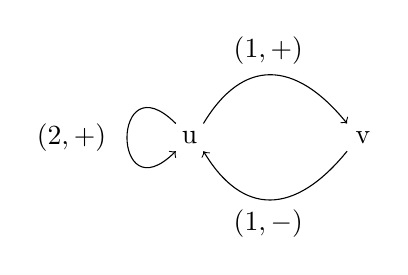
\begin{tikzpicture}
\draw[->] (-5pt,5pt) .. controls (-1,1)  and (-1,-1) .. (-5pt,-5pt);
\node at (0,0) {u};
\node at (2.2,0) {v};
\node at (-1.5,0){$(2,+)$};
\node at (1,1.1){$(1,+)$};
\node at (1,-1.1){$(1,-)$};
\draw[->] (5pt,5pt) .. controls (0.67,1) and (1.33,1) .. (2,5pt);
\draw[->] (2,-5pt) .. controls  (1.33,-1)and (0.67,-1) .. (5pt,-5pt);
\end{tikzpicture}
\end{minipage}
\begin{minipage}[t]{0.45\linewidth}
\centering
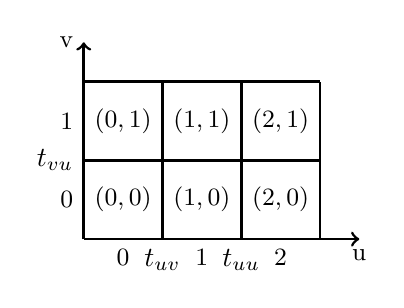
\begin{tikzpicture}[line width=1pt]
\draw[->] (0,0) -- (3.5,0);
\draw[->] (0,0) -- (0,2.5);
\draw[step=1] (0,0) grid (3,2);
\node at (3.5,0)[anchor=north]{\small u};
\node at (0,2.5)[anchor=east]{\small v};
\foreach \x in {0,1,2}
\node at ($(\x,0)+(0.5,0)$)[anchor=north] {\small $\x$};
\foreach \y in {0,1}
\node at ($(0,\y)+(0,0.5)$)[anchor=east] {\small $\y$};
\foreach \x in {0,1,2}
\foreach \y in {0,1}
\node at ($(\x,\y)+(0.5,0.5)$){\small $(\x,\y)$};
\node at (1,0)[anchor=north]{$t_{uv}$};
\node at (2,0)[anchor=north]{$t_{uu}$};
\node at (0,1)[anchor=east]{$t_{vu}$};
\end{tikzpicture}
\end{minipage}
\caption{À gauche : un graphe de régulation ; À droite : l'espace d'états de ce graphe de régulation}\label{figres}
\end{figure}
\end{frame}
\begin{frame}{Approche synchrone et asynchrone}
\begin{figure}[ht]
\begin{minipage}[ht]{0.45\linewidth}
\centering
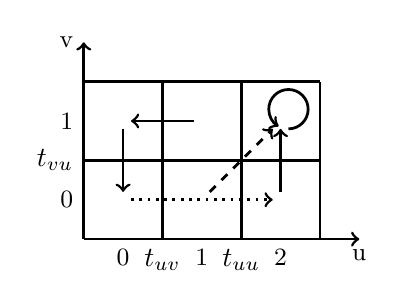
\begin{tikzpicture}[line width=1pt]
\draw[->] (0,0) -- (3.5,0);
\draw[->] (0,0) -- (0,2.5);
\draw[step=1] (0,0) grid (3,2);
\node at (3.5,0)[anchor=north]{\small u};
\node at (0,2.5)[anchor=east]{\small v};
\foreach \x in {0,1,2}
\node at ($(\x,0)+(0.5,0)$)[anchor=north] {\small $\x$};
\foreach \y in {0,1}
\node at ($(0,\y)+(0,0.5)$)[anchor=east] {\small $\y$};
\node at (1,0)[anchor=north]{$t_{uv}$};
\node at (2,0)[anchor=north]{$t_{uu}$};
\node at (0,1)[anchor=east]{$t_{vu}$};
\draw[->] (0.5,1.4) -- (0.5,0.6);
\draw[->] (1.4,1.5) -- (0.6,1.5);
\draw[dotted,->] (0.6,0.5) -- (2.4,0.5);
\draw[dashed,->] (1.6,0.6) -- (2.4,1.4);
\draw[->] (2.5,0.6) -- (2.5,1.4);
\draw[->] (2.6,1.4) arc (-90:240:0.25);
\end{tikzpicture}
\end{minipage}
\begin{minipage}[ht]{0.45\linewidth}
\centering
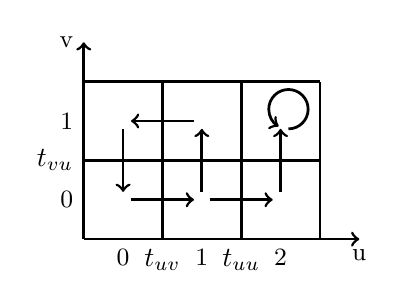
\begin{tikzpicture}[line width=1pt]
\draw[->] (0,0) -- (3.5,0);
\draw[->] (0,0) -- (0,2.5);
\draw[step=1] (0,0) grid (3,2);
\node at (3.5,0)[anchor=north]{\small u};
\node at (0,2.5)[anchor=east]{\small v};
\foreach \x in {0,1,2}
\node at ($(\x,0)+(0.5,0)$)[anchor=north] {\small $\x$};
\foreach \y in {0,1}
\node at ($(0,\y)+(0,0.5)$)[anchor=east] {\small $\y$};
\node at (1,0)[anchor=north]{$t_{uv}$};
\node at (2,0)[anchor=north]{$t_{uu}$};
\node at (0,1)[anchor=east]{$t_{vu}$};
\draw[->] (0.5,1.4) -- (0.5,0.6);
\draw[->] (1.4,1.5) -- (0.6,1.5);
\draw[->] (0.6,0.5) -- (1.4,0.5);
\draw[->] (1.6,0.5) -- (2.4,0.5);
\draw[->] (1.5,0.6) -- (1.5,1.4);
\draw[->] (2.5,0.6) -- (2.5,1.4);
\draw[->] (2.6,1.4) arc (-90:240:0.25);
\end{tikzpicture}
\end{minipage}
\caption{Les attracteurs $K_{v,\omega_v(q)}$ sont les mêmes mais les chemins peuvent être différents}
\end{figure}
\end{frame}
\begin{frame}{Avantages et défauts}
Approche synchrone :
\begin{itemize}
\item Déterministe
\item Possibilité de passer plusieurs niveau dans une transition
\item Possibilité de changer plusieurs variables dans une seule transition
\end{itemize}
\vspace{0.5cm}
Approche asynchrone :
\begin{itemize}
\item Non-déterministe
\item Passage d'un seul niveau dans une transition
\item Au plus une seule variable peut changer par transition
\end{itemize}
\vspace{0.5cm}
Explosion d'espaces d'états
\end{frame}
\section{Process Hitting}
\begin{frame}{Process Hitting}
\begin{figure}
\centering
\tikzscaled[0.8\textwidth]{
%\path[use as bounding box] (0,-1) rectangle (4,4);
%{left, right, top, bottom}
\TSort{(0,0)}{a}{2}{l}
\TSort{(4,0)}{b}{3}{l}
\TSort{(8,0)}{d}{3}{r}
\TSort{(3,-2)}{c}{2}{b}
\THit{a_1}{}{b_1}{.west}{b_0}
\THit{a_0}{}{c_0}{.north}{c_1}
\THit{b_1}{}{a_0}{.east}{a_1}
\THit{c_1}{out=120,in=255}{b_0}{.west}{b_1}
\THit{b_0}{}{d_0}{.west}{d_1}
\THit{b_1}{}{d_1}{.west}{d_2}
\THit{b_2}{bend right=45,in=-30}{d_0}{.east}{d_2}
\THit{d_1}{}{b_0}{.north east}{b_2}
\THit{c_1}{bend right=150,out=-90,in=-90}{d_1}{.south east}{d_0}

\path[bounce,bend right]
\TBounce{b_1}{}{b_0}{.north}
\TBounce{a_0}{}{a_1}{.south}
\TBounce{d_0}{}{d_2}{.south}
\TBounce{b_0}{}{b_2}{.south}
;
\path[bounce,bend left]
\TBounce{d_0}{}{d_1}{.south}
\TBounce{b_0}{}{b_1}{.south}
\TBounce{c_0}{}{c_1}{.west}
\TBounce{d_1}{}{d_2}{.south}
\TBounce{d_1}{}{d_0}{.north}
;
\path[bounce,bend left]
;
\TState{a_0,b_1,c_0,d_0}
}
\caption{Exemple de Process Hitting, sortes : $a,b,c,d$, processus : $a_0,a_1,b_0\ldots$, actions : \ac{a_0}{c_0}{c_1}, \ac{b_1}{a_0}{a_1}$\ldots$)}\label{phex}
\end{figure}
\end{frame}


\begin{frame}{Structure abstraite}
\centerline{Sur-approximation et sous-approximation}
\begin{figure}
\includegraphics[width=0.9\linewidth]{overapp.png}
\caption{La structure abstraite $\mathcal{A}^\omega_\varsigma$ de l'exemple avec l'objectif $d_1\Rsh^*d_2$ et le contexte $\langle a_1,b_0,c_0,d_1\rangle$ , cet objectif n'est pas réalisable.}
\end{figure}
\end{frame}

\section{Complétion}
\subsection{Accessibilité}
\begin{frame}{Fonction de l'outil PINT}
\begin{table}
\begin{tabular}{|c|c|c|}
\hline
Sur-approximation & Sous-approximation & Accessibilité\\
\hline
vrai & vrai & vrai\\
\hline
vrai & faux & inconclusive\\
\hline
faux & vrai & N/A\\
\hline
faux & faux & faux\\
\hline
\end{tabular}
\end{table}
\end{frame}

\begin{frame}{Approches de l'accessibilité \& et de la complétion}
\begin{table}
\begin{tabular}{|c|c|c|c|}
\hline
Méthode & Entrée & Sortie & Calcul\\
\hline 
PINT & processus & non-définitive & non-exhaustif \\ 
\hline 
CSS & séquence & définitive & exhaustif \\ 
\hline 
\end{tabular} 
\end{table}

Résultat de complétion :
\begin{equation}   
\left\{
      \begin{aligned}
             &PINT&+&CP&&inaccessible\to inconclusif/accessible\footnote{CP = Complétion basée sur le processus}\\
             &CSS&&&&inaccessible\to accessible\footnote{CSS = Complétion basée sur la séquence stricte}
      \end{aligned}
\right.  \nonumber
\end{equation}
\end{frame}
\subsection{Complétion basée sur le processus (CP)}
\begin{frame}{Complétion basée sur le processus (CP)}
Éléments :
\begin{itemize}
\item Process Hitting $PH$
\item processus $p$ (inaccessible)
\item ensemble de relations de régulation $R$
\end{itemize}
\end{frame}
\begin{frame}{Classement des processus inaccessibles}
\texttt{unreachableProcess1} : sans actions liées 
$$\{a_i\mid\nexists h=\acm{b_k}{a_j}{a_i}\}$$
\texttt{unreachableProcess2} : avec actions liées
$$\{a_i\mid\exists h=\acm{b_k}{a_j}{a_i}\}$$
\end{frame}
\begin{frame}{Exemple}
$\mathscr{H}=\{\acm{a_1}{b_0}{b_1}\}$, $\varsigma=\{a_0,b_0,c_0\}$, $R=\{(a,b,+),(c,a,-)\}$.\par
\begin{figure}[ht]
\centering
\tikzscaled[0.35\textwidth]{
\coordinate (P1) at (0,0);
\node at (P1) {{\Large c}};
\coordinate (P2) at (2,0);
\node at (P2) {{\Large a}};
\coordinate (P3) at (4,0);
\node at (P3) {{\Large b}};
\coordinate (P4) at ($(P2)+(150:0.6)$);
\draw (P1) circle(0.4) ;
\draw (P2) circle(0.4);
\draw (P3) circle(0.4);
\draw [line width=1pt](30:0.5) .. controls  (1,0.7) .. (P4);
\draw [->, line width=1pt]($(P2)+(30:0.5)$) .. controls  (3,0.7) .. ($(P3)+(150:0.55)$);
\draw [line width=1pt]($(P4)+(45:0.15)$) -- ($(P4)-(45:0.15)$);
}\quad
\tikzscaled[0.55\textwidth]{%[font=\scriptsize]
%\path[use as bounding box] (0,-1) rectangle (4,4);

\TSort{(0,0)}{c}{2}{l}
\TSort{(3,0)}{a}{2}{r}
\TSort{(6,0)}{b}{2}{r}
\THit{a_1}{}{b_0}{.west}{b_1}
\THit{c_0}{color=red}{a_0}{.west}{a_1}


\path[bounce,bend left]
\TBounce{b_0}{}{b_1}{.west}
\TBounce{a_0}{}{a_1}{.west}
;
\TState{a_0,b_0,c_0}
}
\caption{
Au début, $b_1$ n'est pas accessible, comme il a une action liée \ac{a_1}{b_0}{b_1}, $b_1$ est classé dans \texttt{unreachableProcess2}. $a_0$ est évidemment inaccessible car $b_0$ est accessible (état initial). Selon $(c,a,-)\in R$, \ac{c_0}{a_0}{a_1} est rajoutée, alors $b_1$ devient accessible.
}
\end{figure}
\end{frame}
\subsection{Complétion basée sur la séquence stricte (CSS)}
\begin{frame}{Complétion basée sur la séquence stricte (CSS)}
Fonctionnement analogue\par
\vspace{1cm}
Éléments :
\begin{itemize}
\item Process Hitting $PH$
\item séquence stricte $S$
\item ensemble de relations de régulation $R$
\end{itemize}
\end{frame}

\begin{frame}{Exemple}
$\mathscr{H}=\{\acm{b_0}{a_0}{a_1},\acm{a_1}{b_0}{b_1}\}$, le contexte $\varsigma=\{a_0,b_0\}$, ensemble de relations de régulation $R=\{(a,b,+),(b,a,-)\}$. Considérons deux séquences strictes $S_1=a_1::b_1::a_0::b_0$, $S_2=b_1::b_0$
\vspace{0.5cm}
\begin{figure}[ht]
\centering
\begin{tikzpicture}
\TSort{(0,0)}{a}{2}{l}
\TSort{(3,0)}{b}{2}{r}
\THit{a_1}{}{b_0}{.west}{b_1}
\THit{b_0}{}{a_0}{.east}{a_1}
\path[bounce,bend right]
\TBounce{a_0}{}{a_1}{.south east}
;
\path[bounce,bend left]
\TBounce{b_0}{}{b_1}{.west}
;
\TState{a_0,b_0}
\end{tikzpicture}
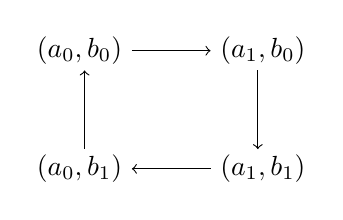
\begin{tikzpicture}
\coordinate (P1) at (0,0);
\coordinate (P2) at (1,0);
\coordinate (P3) at (1,-1.5);
\coordinate (P4) at (0,-1.5);
\node at (P1)[anchor=east]{$(a_0,b_0)$};
\node at (P2)[anchor=west]{$(a_1,b_0)$};
\node at (P3)[anchor=west]{$(a_1,b_1)$};
\node at (P4)[anchor=east]{$(a_0,b_1)$};
\draw[->](P1)--(P2);
\draw[<-](-0.6,-0.25)--(-0.6,-1.25);
\draw[->](P3)--(P4);
\draw[->](1.6,-0.25)--(1.6,-1.25);
\end{tikzpicture}
\end{figure}
\end{frame}
\begin{frame}{Approches de l'accessibilité \& et de la complétion}
\begin{table}
\begin{tabular}{|c|c|c|c|}
\hline
Méthode & Entrée & Sortie & Calcul\\
\hline 
PINT & processus & non-définitive & non-exhaustif \\ 
\hline 
CSS & séquence & définitive & exhaustif \\ 
\hline 
\end{tabular} 
\end{table}

Résultat de complétion :
\begin{equation}   
\left\{
      \begin{aligned}
             &PINT&+&CP&&inaccessible\to inconclusif/accessible\footnote{CP = Complétion basée sur le processus}\\
             &CSS&&&&inaccessible\to accessible\footnote{CSS = Complétion basée sur la séquence stricte}
      \end{aligned}
\right.  \nonumber
\end{equation}
\end{frame}
\begin{frame}{Conclusion}
\begin{enumerate}
\item Propriété du Process Hitting\cite{Pauleve2014,pauleve2011modelisation,Pauleve2012}
\item Contribution au Process Hitting (cut set\cite{Pauleve2013} \& complétion)
\item Avantages
\begin{itemize}
\item Données imprécises
\item Complexité réduite
\end{itemize}
\item Défauts
\begin{itemize}
\item Construction de $R$
\item Sémantiques manquantes
\end{itemize}
\end{enumerate}
\end{frame}

\begin{frame}[allowframebreaks]{Références}
%\beamertemplatetextbibitems
\renewcommand\refname{Références}
\bibliographystyle{plain}
\bibliography{MasterBib}


\end{frame}
\end{document}